\documentclass{beamer}

\usepackage{fancyvrb}
\usepackage{color, colortbl}
\usepackage{listings}
\usepackage{url}
\usepackage{array}
\usepackage{calc}
\usepackage{ctable}
\usepackage{amsmath}
\usepackage{cite}
\usepackage{graphicx}
\usepackage{listings}
\usepackage{xspace}
\usepackage{hyperref}
\usepackage{subfigure}
\usepackage{multicol}
\definecolor{lightgray}{rgb}{0.9,0.9,0.9}



\lstset{ %
language=C++,                % choose the language of the code
basicstyle=\tiny,       % the size of the fonts that are used for the code
%numbers=left,                   % where to put the line-numbers
numbers=none,                   % where to put the line-numbers
numberstyle=\scriptsize,      % the size of the fonts that are used for the line-numbers
stepnumber=1,                   % the step between two line-numbers. If it's 1 each line will be numbered
numbersep=15pt,                  % how far the line-numbers are from the code
backgroundcolor=\color{lightgray},  % choose the background color. You must add \usepackage{color}
%backgroundcolor=none,  % choose the background color. You must add \usepackage{color}
showspaces=false,               % show spaces adding particular underscores
showstringspaces=false,         % underline spaces within strings
showtabs=false,                 % show tabs within strings adding particular underscores
frame=single,	                % adds a frame around the code
%frame=none,	                % adds a frame around the code
tabsize=2,	                % sets default tabsize to 2 spaces
%captionpos=b,                   % sets the caption-position to bottom
captionpos=n,
%basicstyle=\small,
%basicstyle=\small\sffamily,
basicstyle=\sffamily\small,
%basicstyle=\ttfamily\small,
breaklines=true,                % sets automatic line breaking
breakatwhitespace=false,        % sets if automatic breaks should only happen at whitespace
columns=fullflexible,
title=\lstname,                 % show the filename of files included with \lstinputlisting; also try caption instead of title
escapeinside={\%*}{*)},          % if you want to add a comment within your code
morekeywords={chare,mainchare,module,mainmodule,entry,readonly,array,serial,for,when,if,then,else,overlap,while,forall,threaded,sync,message},
aboveskip=2pt,
belowskip=2pt,
lineskip=0pt,
xleftmargin=1em,
xrightmargin=1em,
%xleftmargin=10pt
abovecaptionskip=0pt,
belowcaptionskip=0pt,
}

\hypersetup{
    colorlinks,%
    citecolor=black,%
    filecolor=black,%
    linkcolor=black,%
    urlcolor=magenta
}


\newcommand{\charm}{Charm++}
\newcommand{\code}[1]{\colorbox{lightgray}{\texttt{#1}}}
\newcommand{\transition}[1]{\begin{frame}[plain]\begin{center}\LARGE #1\end{center}\end{frame}}
\newcommand{\comment}[1]{ }
\newcommand{\eat}[1]{ }

\DefineVerbatimEnvironment{codeverb}{Verbatim}{fontsize=\small}

\let \isForClass 1
\if \isForClass 1
  \newcommand{\removeForClass}[2]{#2}
  \else
  \newcommand{\removeForClass}[2]{#1}
\fi


\usefonttheme{professionalfonts}

\usetheme{Boadilla}
\usecolortheme{beaver}

\AtBeginSection[]{
}

\title[Parallelism with Charm++]{Parallel Programming with \charm}
\institute[PPL, UIUC]{\includegraphics[scale=0.8]{../figures/illinois_logo-crop.pdf}\\Parallel Programming Lab\\ University of Illinois}
\author[Phil and Ram]{Phil Miller, Ramprasad Venkataraman, Laxmikant Kal\'e}
\date{May 14, 2012}

\begin{document}

\frame{\titlepage}

\section{Why Parallelism}
\section{Motivating Challenges}
\begin{frame}
\frametitle{Audience Poll: Challenges of Parallel Programming}
How many of you have written parallel programs that suffer from:
\begin{itemize}[<+->]
\only<1>{\item Bad scaling?
\includegraphics{../figures/bad_scalability.pdf}}
\only<2>{\item Sad scaling?
\includegraphics{../figures/sad_scalability.pdf}}
\item Bad scaling?
\item Races, deadlocks, etc: gremlins of shared state?
\pause
\item Limited to shared memory? GPU? No sharing allowed?
\item Coded to match core count?
\only<6>{
\item Independent tasks serialized or badly split across resources?
\includegraphics[width=.45\textwidth]{../figures/timeDivision.pdf}\\
\includegraphics[width=.45\textwidth]{../figures/spaceDivision.pdf}
}
\item Independent tasks serialized or badly split across resources?
\item Application logic interwoven with parallelism optimizations?
\item Wasted energy?
\item Square-peg logic in round-hole framework abstractions?
\end{itemize}
\end{frame}

\section{\charm}
\begin{frame}
\frametitle{\charm}
\framesubtitle{}
    \begin{itemize}
        \item description
    \end{itemize}
\end{frame}


\begin{frame}
\frametitle{\charm: Some Capabilities}
\framesubtitle{}
    \begin{itemize}
        \item -
    \end{itemize}
\end{frame}


\begin{frame}
\frametitle{\charm: Portability}
\framesubtitle{}
    \begin{itemize}
        \item -
    \end{itemize}
\end{frame}



\section{Expressing Parallel Algorithms}
\begin{frame}
  \frametitle{Express Parallel Algo independent of processors}
  \begin{figure}\includegraphics[width=0.9\textwidth]{../figures/progmodel/01-objects-for-algo.pdf}\end{figure}
\end{frame}


\begin{frame}
  \frametitle{Data Decomposition via Collections of Objects}
  \begin{figure}\includegraphics[width=0.9\textwidth]{../figures/progmodel/02-data-decomp-via-arrays.pdf}\end{figure}
\end{frame}


\begin{frame}
  \frametitle{Multiple data parallel control flows}
  \begin{figure}\includegraphics[width=0.9\textwidth]{../figures/progmodel/03-many-data-parallel-arrays.pdf}\end{figure}
\end{frame}


\begin{frame}
  \frametitle{Decompose parallel functionality into interacting classes}
  \begin{figure}\includegraphics[width=0.9\textwidth]{../figures/progmodel/04-func-decomp-via-classes.pdf}\end{figure}
\end{frame}


\begin{frame}
  \frametitle{
    \only<1>{Parallelism requires distributing objects across processors}
    \only<2>{However, do not burden programmer with this view}
  }
  \begin{figure}\includegraphics[width=0.9\textwidth]{../figures/progmodel/05-objects-sys-view.pdf}\end{figure}
\end{frame}


\begin{frame}
  \frametitle{
    \only<1>{Elevate some objects to global visibility}
    \only<2>{Addressing objects is independent of location}
  }
  \begin{figure}\includegraphics[width=0.9\textwidth]{../figures/progmodel/06-elevate-obj-2-global-space.pdf}\end{figure}
\end{frame}


\begin{frame}
    class / object - fundamental unit of state natural to parallel algo\\
    method - fundamental unit of execution in parallel algo\\
    express parallel algo interactions via methods or function calls
\end{frame}


\begin{frame}
  \frametitle{Objects interact via methods}
  \begin{figure}
    \includegraphics[width=0.9\textwidth]{../figures/progmodel/07-algo-via-objects-methods.pdf}
  \end{figure}
\end{frame}



\section{Asynchronous RMI}
\begin{frame}
  \frametitle{Object Interactions \only<4>{ ... via remote method invocations}}
  \begin{figure}
%so far we only spoke abt units of state in the app
%and expressing the app in terms of units natural to the domain
%so we've done that.
	\includegraphics<1>[width=0.9\textwidth]{../figures/progmodel/07-obj-programmer-view.pdf}
%we have this impressive decomposition of data and functionality across collections of objects
%how do you stitch all these objects into a cohesive fabric that makes the app do what its supposed to do
%there's one ingredient that i've avoided mentioning up to this point and those are interactions.
%these obj have to interact with each other
	\includegraphics<2>[width=0.9\textwidth]{../figures/progmodel/05-parallelism-via-obj-collections.pdf}
%in a sequential environment, which all of us are familiar with
%app state is in objects, and app logic / interactions is via method invocations
	\includegraphics<3>[width=0.9\textwidth]{../figures/progmodel/08-seq-obj-methods.pdf}
%charm retains this same modality
%we enable method invocations across process or addr space boundaries
%however with minor modifications from the sequential semantic
	\includegraphics<4>[width=0.9\textwidth]{../figures/progmodel/09-rmi-synchronous.pdf}
  \end{figure}
\end{frame}


\begin{frame}
\frametitle{1. Not every object is remotely invocable}
%we do NOT encourage a notion of a flat global address space, where it magically appears that
%all app entities are in the same address space, and any object can call / interact with anyone else
%instead, we strive to keep the locality information visible to the app
%the first step to that is to permit RMI only on globally visible objects
  \begin{figure}\includegraphics[width=0.9\textwidth]{../figures/progmodel/10-rmi-notgas.pdf}\end{figure}
\end{frame}


\begin{frame}
\frametitle{2. Not every method is remotely invocable}
%only subset of methods elevated into global namespace
%programmer annotates which methods are globally visible
%only globally visible methods can be invoked across proc boundaries
%intro term entry methods. will explain why later.
  \begin{figure}\includegraphics[width=0.9\textwidth]{../figures/progmodel/11-global-methods.pdf}\end{figure}
\end{frame}


\begin{frame}
\frametitle{3. Remote methods are of void return type}
  What happens if an object waits for a return value from a method invocation?
  \pause
  \begin{center}
    \includegraphics[width=\textwidth]{../figures/objectSequence.pdf}
  \end{center}
  \pause
  \begin{itemize}
    \item Performance
    \item Latency
    \item Reasoning about correctness
  \end{itemize}
\end{frame}


\begin{frame}
\frametitle{3. Remote methods are of void return type}
  \begin{center}
    \includegraphics[width=\textwidth]{../figures/objectSequenceAsync.pdf}
  \end{center}
  \begin{itemize}
  \item Hence, method invocations should be asynchronous
    \begin{itemize}
    \item No return values
    \end{itemize}
  \item Computations are driven by the incoming data
    \begin{itemize}
    \item Initiated by the sender or method caller
    \end{itemize}
  \end{itemize}
\end{frame}


\begin{frame}
\frametitle{3. Remote methods are of void return type}
	\onslide<2>{ Asynchronous, non-blocking remote method invocations }
	\begin{center}
        \includegraphics<1>[width=0.9\textwidth]{../figures/progmodel/11-global-methods.pdf}
        \includegraphics<2>[width=0.9\textwidth]{../figures/progmodel/12-async-nonblock-rmi.pdf}
	\end{center}
\end{frame}


\begin{frame}
\frametitle{How do you get return values}
	\begin{center}
        \includegraphics[width=0.9\textwidth]{../figures/progmodel/13-rmi-return-values.pdf}
	\end{center}
\end{frame}


\begin{frame}
\frametitle{Collective addressing of object collections}
	\begin{center}
        \includegraphics[width=0.9\textwidth]{../figures/progmodel/14-rmi-collective.pdf}
	\end{center}
\end{frame}


\begin{frame}
\frametitle{RMI expresses parallel dependencies}
	\begin{center}
        lu DAG?
        \includegraphics[width=0.9\textwidth]{../figures/progmodel/11-global-methods.pdf}
	\end{center}
\end{frame}




\section{Execution Model}
\begin{frame}
\frametitle{ RMI $\rightarrow$ Messages }
	\begin{center}
        % so how do we achieve RMI. method invocations are transmitted to remote locations as messages
        \includegraphics<1>[width=0.9\textwidth]{../figures/progmodel/14-rmi-collective.pdf}
        % but they're completely asynchronous. no ack / assent required from receiving processor
        % hence, a processor could receive multiple remote methods simultaneously for execution
        % so how do we handle this
	\end{center}
\end{frame}


\begin{frame}
\frametitle{Remember the void return types?}
    \begin{itemize}
        \item \alert{void return types imply one-way information transfer}
        \item signal application's intent to perform (possibly) remote task
        \item carry required input data for remote task
        \item \alert{express parallel dependencies}
        \pause
        \begin{block}{}
            Entry methods express when something \alert{can} execute.\\
            Not when something \alert{should} execute.
        \end{block}
    \end{itemize}
\end{frame}


\begin{frame}
\frametitle{
    \only<1>{ RMI $\rightarrow$ Messages }
    \only<2>{ Message queues }
    \only<3>{ Scheduler }
}
	\begin{center}
        % so how do we achieve RMI. method invocations are transmitted to remote locations as messages
        \includegraphics<1>[width=0.9\textwidth]{../figures/progmodel/14-rmi-collective.pdf}
        % the natural way to handle this is to use a msg q
        % so this introduces the first component at the runtime layer. above line is app. below line is rts
        % charm maintains a msg queue under the hood to handle all the msgs that comprise parallel execution
        \includegraphics<2>[width=0.9\textwidth]{../figures/progmodel/15-msg-queues.pdf}
        % how is parallel execution actually orchestrated?
        % remember that all methods are completely one-way info flows. once an RMI is packaged into a msg,
        % it has everything thats needed from the sender. this means, it can basically be invoked anytime.
        % so msgs can be picked out of this queue, the receiving object identified
        % and the method invocation can be executed
        % This is performed by the runtime scheduler. which is the engine that drives the whole parallel execution
        \includegraphics<3>[width=0.9\textwidth]{../figures/progmodel/16-scheduler.pdf}
	\end{center}
\end{frame}


\begin{frame}
\frametitle{\charm}
\begin{itemize}
    \item objects = fundamental unit of state / functionality
    \item methods = fundamental unit of execution
\end{itemize}
\pause
\begin{block}{Entry Methods ...}
\begin{itemize}[<+->]
    \item are \emph{scheduled} for execution
    \item are not preempted
    \item are not reentrant
    \item have unspecified delivery order
    \item do not require threading / locking mechanisms (typically)
\end{itemize}
\end{block}
\end{frame}


\begin{frame}
\frametitle{Prioritized Execution}
	\begin{center}
        \includegraphics<1>[width=0.9\textwidth]{../figures/progmodel/16-scheduler.pdf}
        \includegraphics<2>[width=0.9\textwidth]{../figures/progmodel/17-prio-scheduling.pdf}
	\end{center}
\end{frame}



\begin{frame}
\frametitle{Cosmology: ChaNGa}
\begin{center}
\includegraphics[width=0.9\textwidth]{../figures/changa-length-scales.pdf}
\end{center}
\end{frame}


\begin{frame}
\frametitle{Cosmology: ChaNGa}
\begin{center}
\includegraphics[width=0.9\textwidth]{../figures/changa.pdf}
\end{center}
\end{frame}


\begin{frame}
\frametitle{Cosmology: ChaNGa}
\begin{center}
\includegraphics[width=0.9\textwidth]{../figures/changa-scaling.pdf}
\end{center}
\end{frame}



\section{Decomposition and Grain Size}
\begin{frame}
\frametitle{Parallel Decomposition}
\framesubtitle{Recap}
\begin{itemize}
\item Data or Task parallelism encoded in objects
\item Object count independent of processors
\item How many objects, then? How big?
\end{itemize}
\end{frame}

\begin{frame}
\frametitle{Parallel Decomposition}
\framesubtitle{Overdecomposition}
Want \emph{several} objects per processor
\begin{itemize}
\item Increase chance that one will have work available
\item Overlap communication of one with computation of another
\item Important for later optimizations
\end{itemize}
\end{frame}

\begin{frame}[fragile]
\frametitle{Parallel Decomposition}
\framesubtitle{Overdecomposition Example: Weather Forecasting in BRAMS}
\begin{itemize}
 \item BRAMS: Brazillian weather code (based on RAMS)
 \item AMPI version (Eduardo Rodrigues, with C. Mendes and J. Panetta)
\end{itemize}
\includegraphics[width=0.9\textwidth]{../figures/bramsVisual.png}
\end{frame}


\begin{frame}[fragile]
\frametitle{Basic Virtualization of BRAMS}
\includegraphics[width=0.5\textwidth]{../figures/bramsNonVirtual.png}
\includegraphics[width=0.5\textwidth]{../figures/bramsVirtual.png}
\end{frame}

\begin{frame}[fragile]
\frametitle{Baseline: 64 objects on 64 processors}
\begin{center}\includegraphics[width=0.9\textwidth]{../figures/usageNonVirtual.png}\end{center}
\end{frame}

\begin{frame}[fragile]
\frametitle{Over-decomposition: 1024 objects on 64 processors}
\framesubtitle{Benefits from communication/computation overlap}
\begin{center}\includegraphics[width=0.9\textwidth]{../figures/usageVirtual.png}\end{center}
\end{frame}


\begin{frame}
\frametitle{Grain Size}
  \begin{block}{Working Definition} The amount of computation per potentially
      parallel event (task creation, enqueue/dequeue, messaging,
      locking, etc.)
  \end{block}
  \begin{center} \includegraphics[width=0.7\textwidth]{../figures/grain1.png} \end{center}
\end{frame}

\section{Modularity and Composability}
\begin{frame}
\frametitle{Modularity \& Composability}
\begin{itemize}
\item Easy to write code separately and then run it separately
\includegraphics[width=.45\textwidth]{../figures/timeDivision.pdf}
\includegraphics[width=.45\textwidth]{../figures/spaceDivision.pdf}
\item Possible to write code for explicit paralllel composition, interleaving multiple modules
\item Want seamless resource sharing by separate pieces of code
\includegraphics[width=.7\textwidth]{../figures/composition.pdf}
\end{itemize}
\end{frame}

\section{Separation of Concerns}
\begin{frame}
\frametitle{Separation of Concerns}
\begin{block}{Different expertise, different focus}
Relevant pieces of code should be easy to divide
\end{block}
\begin{itemize}
\item Much like any library -- clients control behavior by passing
  arguments, not modifying implementation
\item Can be very flexible -- arguments with behavior of their own
  (e.g., functors)
\item Several examples: initial mapping schemes, dynamic load
  balancing strategies
\item CS-specialist logic doesn't pollute application code, can be
  swapped out with minimal effort
\item Location-independent algorithm expression and runtime-mediated
  execution are essential enabling features
\end{itemize}
\end{frame}


\begin{frame}
\frametitle{Different expertise, different focus}
\framesubtitle{Mapping Example: Quantum Chemistry with {\sc OpenAtom}}
Replace with illustration of OpenAtom arrays
\end{frame}

\begin{frame}
\frametitle{Different expertise, different focus}
\framesubtitle{Mapping Example: Quantum Chemistry with {\sc OpenAtom}}
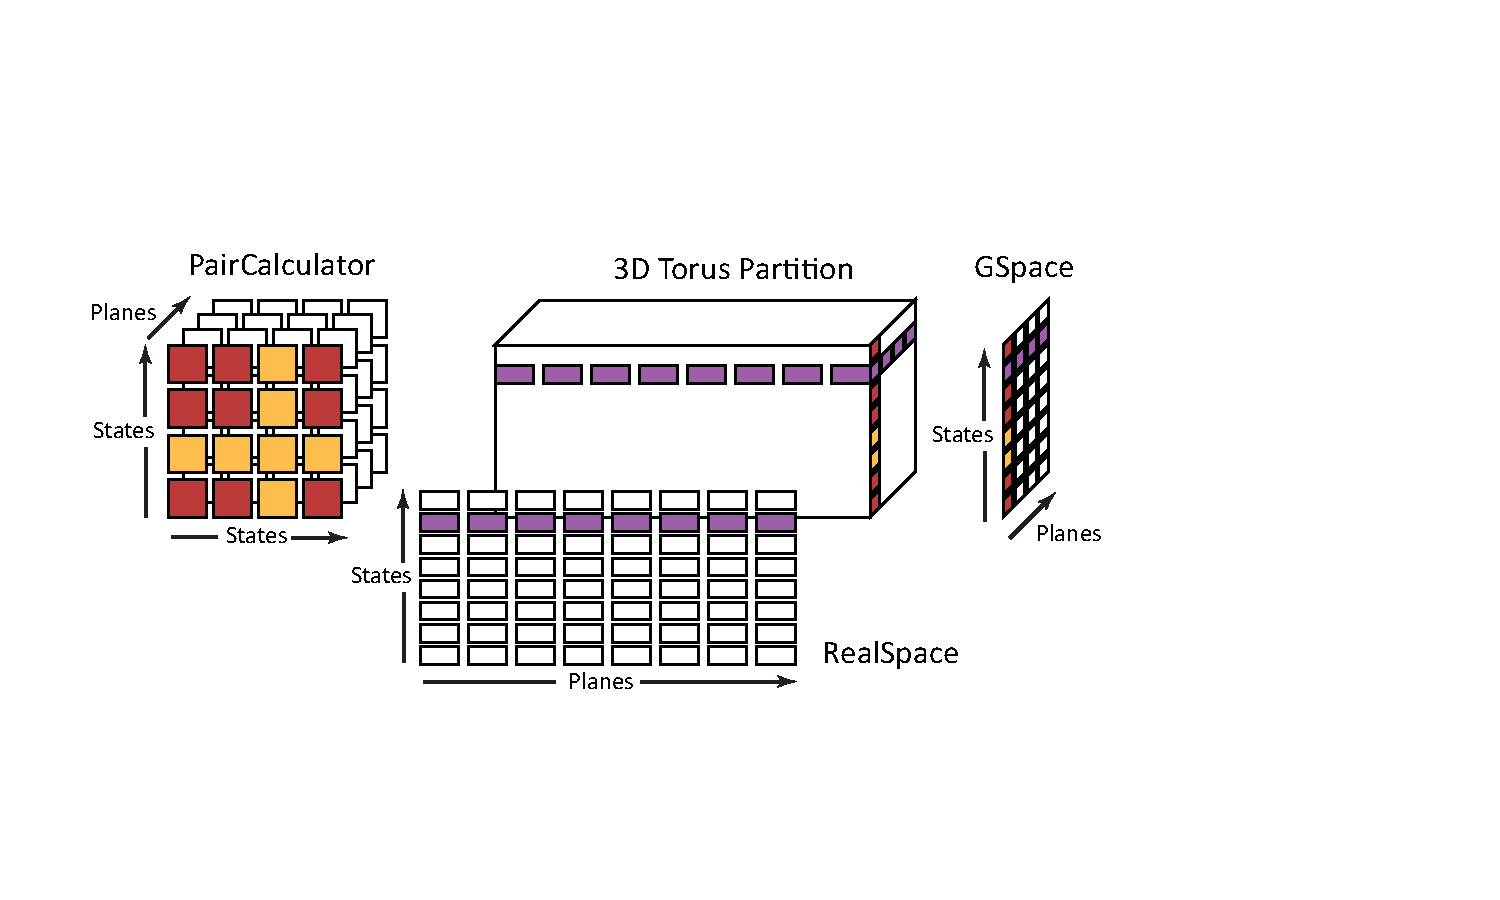
\includegraphics[width=0.9\textheight]{../figures/openatom/mapping.pdf}
\end{frame}


\begin{frame}
\frametitle{Different expertise, different focus}
\framesubtitle{Mapping Example: Quantum Chemistry with {\sc OpenAtom}}
\includegraphics[width=0.9\textwidth]{../figures/openatom/map.pdf}
\begin{block}{40\% improvement, application only changed in initialization!}\end{block}
\end{frame}


\begin{frame}
\frametitle{Separation of Concerns}
\begin{block}{Layered responsibility}
Application worries about \emph{what}, runtime system worries about \emph{how}
\end{block}
\begin{itemize}
\item What data to send, vs. message allocation and packing
\item Who to talk to, vs. where they live
\end{itemize}
\end{frame}

\begin{frame}
\frametitle{Separation of Concerns}
\framesubtitle{Example: Object location services}
\begin{itemize}[<+->]
\item Possible solutions to ``Where does object X live?''
\begin{itemize}[<+->]
\item Name is location-specific
\item Creator specifies location, passes along with name
\item Fixed mapping from names to locations
\item \textbf{Dynamic lookup}
\end{itemize}
\item \charm approach
\begin{itemize}
\item \emph{Mapping scheme} defines \emph{home location} -- default location, and responsible for knowing current location
\item Cache of last known locations on each processor
\item Messages sent to cached location, or home if none known
\end{itemize}
\end{itemize}
\pause
\begin{block}{Application is mostly oblivioous}
Fire off message, runtime delivers
\end{block}
\end{frame}

\section{Introspective, Adaptive Runtime System}
\begin{frame}
\frametitle{Introspective, Adaptive Runtime System}
All about execution resources: processors, network, nodes, etc.
\begin{itemize}
\item Watch how each object and method uses resources: time running, bytes/messages sent & received, CPU frequency sensitivity, performance counters
\item Record instrumented data for other components to use
\item Invoke adaptation mechanisms at appropriate intervals
\item Adjust system configuration accordingly
\end{itemize}
\end{frame}




\begin{frame}
\frametitle{Load Imbalance}
\begin{itemize}
\item Performance limited by difference between most-loaded processor and overall average.\\
\only<1>{\includegraphics[width=0.8\textwidth]{../figures/changa_imbalance.png}}
\pause
\item Causes vary in severity, time scale, nature
\pause
\item Response must suit causes, other application concerns, system scale
\end{itemize}
\end{frame}


\begin{frame}[fragile]
\frametitle{Load Imbalance: Crack Propagation}
\begin{columns}
\begin{column}{0.5\textwidth}
\includegraphics[width=\textwidth]{../figures/chunkGraph16}
\end{column}
\begin{column}{0.5\textwidth}
Decomposition into 16 chunks using Metis. The middle area contains cohesive elements.

As computation progresses, crack propagates, and new elements are added, leading to more complex computations in some chunks

Picture: S. Breitenfeld and P. Geubelle
\end{column}
\end{columns}
\end{frame}

\begin{frame}[fragile]
\frametitle{Load Balancing Crack Propagation}
\begin{centering}
\includegraphics[width=1.0\textwidth]{../figures/LButilizationCrackPropWithAnnotation}
\end{centering}
\end{frame}


\begin{frame}
\frametitle{Adaptive Mesh Refinement for solving PDEs}
\includegraphics[width=0.9\textwidth]{../figures/amr_scaling_distlb.pdf}
\end{frame}





\begin{frame}
\frametitle{Power, Energy, and Heat}
\framesubtitle{Motivations}
\begin{itemize}
\item Reduce direct costs of execution - cumulative machine energy, cooling energy from start to finish
\item Reduce capital costs - transformers, chillers
\item Improve reliability
\item Improve user experience - fan noise, ambient heat, battery life
\end{itemize}
\end{frame}

\begin{frame}[t]
\frametitle{Power, Energy, and Heat}
\begin{block}{Established Technique}
Set temperature threshold, periodic DVFS to enforce
\end{block}
\begin{itemize}
\item Slower clocks can hurt performance
\item Load balance to compensate
\end{itemize}
\includegraphics[width=0.3\textwidth]{../figures/ft_par.pdf}
\includegraphics[width=0.3\textwidth]{../figures/jacobi_par.pdf}
\includegraphics[width=0.3\textwidth]{../figures/wave_par_bk.pdf}
\pause
\begin{block}{Upcoming Technique}
Set power threshold on newer Intel CPUs, load balance as overloads appear
\end{block}
\end{frame}



\input{ft}
\section{Scalability}
\begin{frame}
\frametitle{Computational Biomolecular Physics: NAMD}
\includegraphics[width=0.9\textwidth]{../figures/namd/chromatophore-vesicle-2012-01.jpg}
\end{frame}


\begin{frame}
\frametitle{Biomolecular Physics: NAMD}
\includegraphics[width=0.9\textwidth]{../figures/namd_bgp.pdf}
\end{frame}


\begin{frame}
\frametitle{Biomolecular Physics: NAMD}
\includegraphics[width=0.9\textwidth]{../figures/namd_titan.pdf}
\end{frame}


\begin{frame}
\frametitle{Cosmology: ChaNGa}
\includegraphics[width=0.9\textwidth]{../figures/changa-length-scales.pdf}
\end{frame}


\begin{frame}
\frametitle{Cosmology: ChaNGa}
\includegraphics[width=0.9\textwidth]{../figures/changa-scaling.pdf}
\end{frame}


\begin{frame}
\frametitle{Quantum Chemistry: OpenAtom}
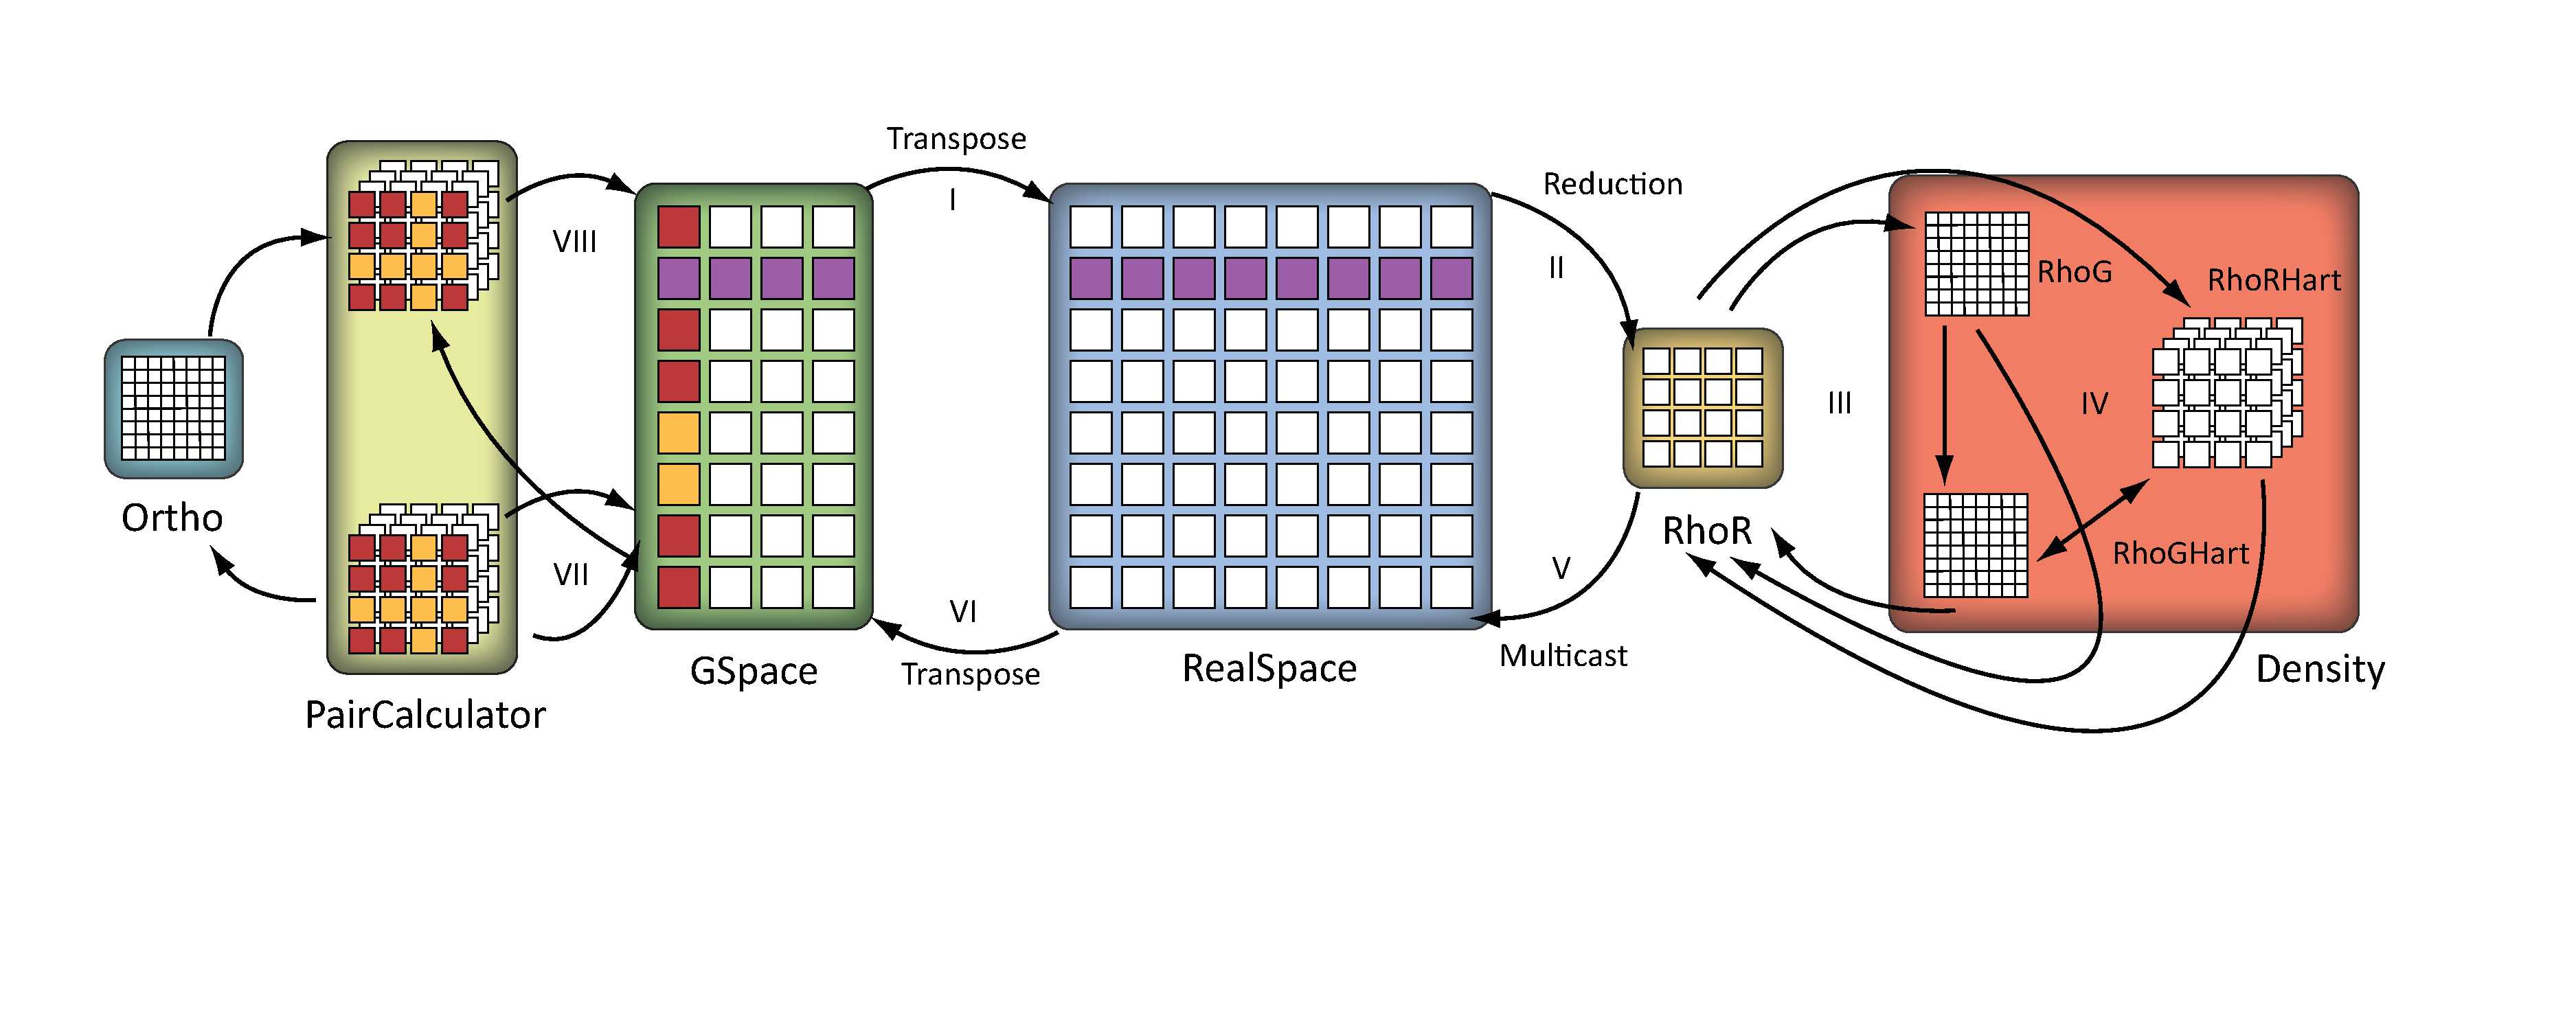
\includegraphics[width=0.45\textheight]{../figures/openatom/control-flow.pdf}
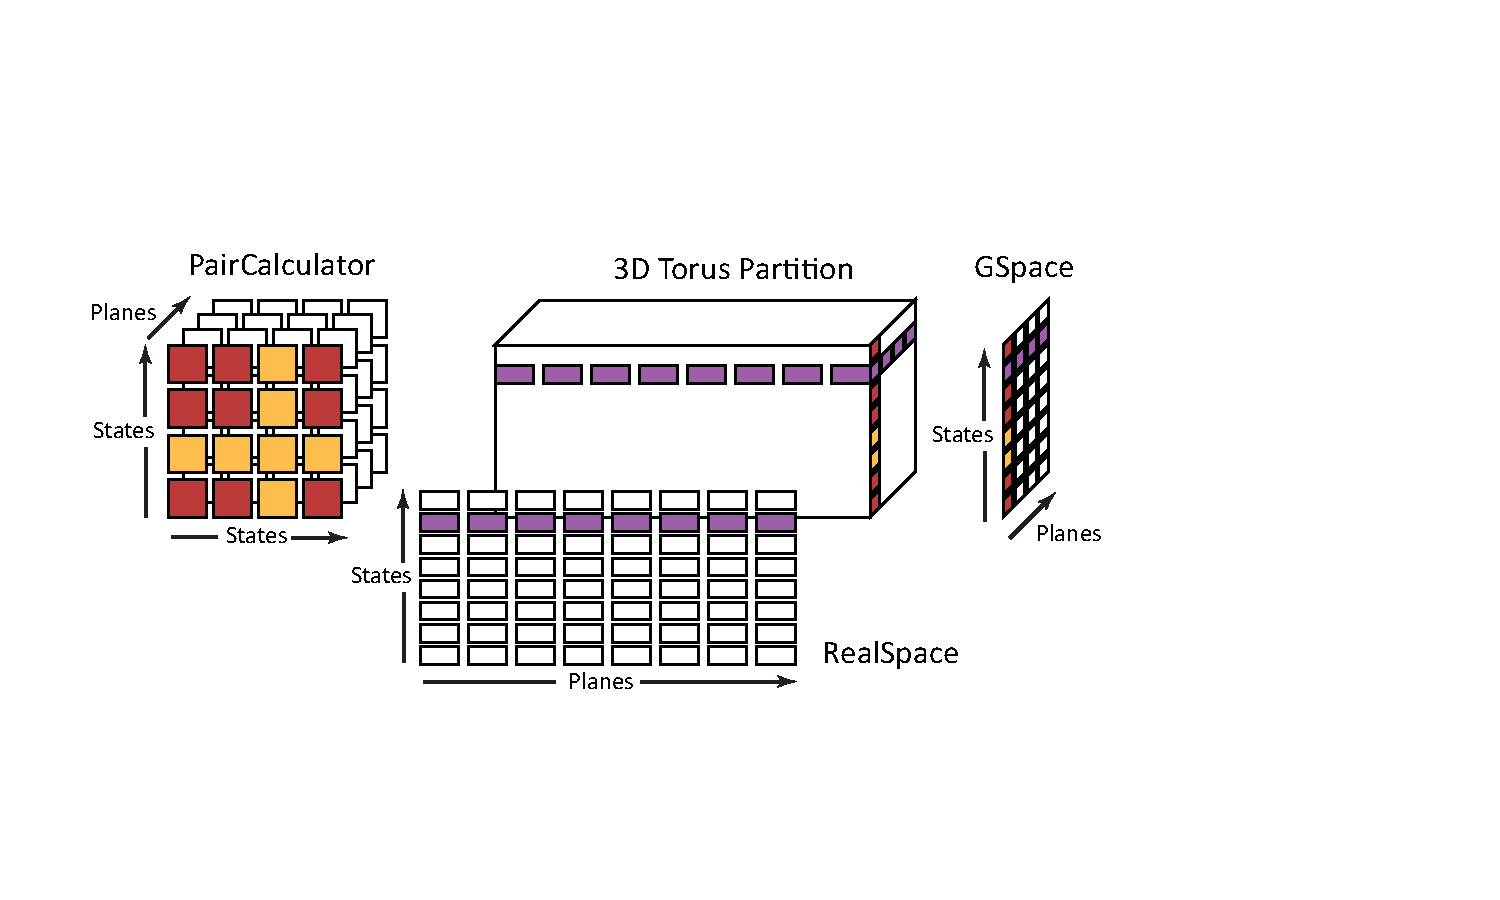
\includegraphics[width=0.45\textheight]{../figures/openatom/mapping.pdf}
\end{frame}


\begin{frame}
\frametitle{Quantum Chemistry: OpenAtom}
\includegraphics[width=0.9\textwidth]{../figures/openatom/bgq.pdf}
\end{frame}


\begin{frame}
\frametitle{Contagion and Information Spread: CharmEpiSimDemics}
\includegraphics[width=0.9\textwidth]{../figures/contagion.png}
\end{frame}


\begin{frame}
\frametitle{Contagion and Information Spread: CharmEpiSimDemics}
\includegraphics[width=0.9\textwidth]{../figures/simdemics_strong_scaling.pdf}
\end{frame}


\begin{frame}
\frametitle{JetAlloc}
%
\begin{itemize}
\item
\end{itemize}
%
%\includegraphics{../figures/}
\end{frame}

\begin{frame}
\frametitle{AMR}
%
\begin{itemize}
\item
\end{itemize}
%
\includegraphics[scale=0.7]{../figures/amr_scaling_distlb.pdf}
\end{frame}

\begin{frame}
\frametitle{kdTree SMP}
\begin{itemize}
\item
\end{itemize}
%
%\includegraphics{../figures/}
\end{frame}

\begin{frame}
\frametitle{Numerical Linear Algebra}
%
Sparse Triangular Solver vs. SuperLU\_Dist
\includegraphics[scale=0.45]{../figures/sparselu_superlu_comparison.pdf}\\
Dense factorization: CharmLU
\includegraphics[scale=0.2]{../figures/charmlu_scaling.pdf}
\end{frame}


\section{Tooling}
\begin{frame}
  \frametitle{Performance Analysis Using Projections}
  \begin{block}{Instrumentation and measurement during program execution}
    \begin{itemize}
        \item Easy setup: just modify link options
        \item Easy setup: data is generated automatically during run
        \item User events can be easily inserted as needed
    \end{itemize}
  \end{block}
  \begin{block}{Visualization and analysis client}
    \begin{itemize}
        \item Scalable: analyze execution traces for 100s of thousands of cores 
        \item Rich feature set: time profile, time lines, usage profile, histograms, outliers etc
        \item Detect performance problems: load imbalance, grain size, communication bottleneck, etc 
    \end{itemize}
  \end{block}
\end{frame}


\begin{frame}{Time Profile}
 \includegraphics<1>[width=0.9\textwidth]{../figures/prj1M8KTimeprofile.png}
\end{frame}

\begin{frame}{Extrema Tool for Least Idle Processors}
\includegraphics<1>[width=0.9\textwidth]{../figures/prj1M8KExtrema.png}
\end{frame}

\begin{frame}{Time Lines with Message Back Tracing}
\centering
\includegraphics<1>[width=0.9\textwidth]{../figures/prj1M8KTimeline.png}
\end{frame}


\begin{frame}{Communication over Time for all Processors}
 \includegraphics<1>[width=0.9\textwidth]{../figures/prj1M8KCommtime.png}
\end{frame}


\begin{frame}[fragile]
  \frametitle{Debugging \charm applications using CharmDebug}
  \begin{center}\includegraphics[width=0.9\textwidth]{../figures/overviewDebug.png}\end{center}
\end{frame}

\begin{frame}[fragile]
  \frametitle{Debugging \charm applications using CharmDebug}
  \begin{center}\includegraphics[width=0.9\textwidth]{../figures/debugMainView.png}\end{center}
\end{frame}


\section{Recap}
\begin{frame}
\frametitle{Recap}
\includegraphics[width=\textwidth]{../figures/charmwebsite-screenshot.png}
\end{frame}


\begin{frame}
\frametitle{Questions?}
\includegraphics[width=\textwidth]{../figures/charmOutline.png}
\end{frame}


\end{document}

